\section{Zielsetzung}
Im Versuch wird die Elektronenstrahlablenkung sowohl im elektrischen, als auch im
magnetischen Feld untersucht.

\section{Theorie}
\subsection{Erzeugung eines Elektronenstrahls}
Um einen Elektronenstrahl zu erzeugen, wird im Versuch eine sogenannte Kathodenstrahlröhre
verwendet. Diese besteht prinzipiell aus verschiedenen Komponenten, die in Abblidung \ref{abb1}
schematisch dargestellt sind. Der Elektronenstrahl wird hier über einen erhitzten Draht emittiert,
dessen Intensität vom Wehneltzylinder geregelt werden kann. Direkt dahinter befinden sich
eine Elektrode, die dazu dient, den Elektronenstrahl zu beschleunigen. Die darauf folgenden
Elektroden dienen zur Bündelung und Fokussierung des Elktronenstrahls. Zum Schluss,
vor dem Detektorschirm befinden sich zwei Plattenpaare, zwischen denen, mittels einer angelegten
Spannung, elektrische Felder entstehen, die den Elektronenstrahl zum einen horizontal (x-Richtung) und
zum anderen vertikal (y-Richuntg) ablenken können. Danach trifft der Strahl auf einen Detektorschirm, welcher
die physikalischen Eigenschaften besitzt, den auftreffenden Elektronenstrahl in Fornm eines
Leuchtflecks sichtbar zu machen.
\FloatBarrier
\begin{figure}
  \centering
  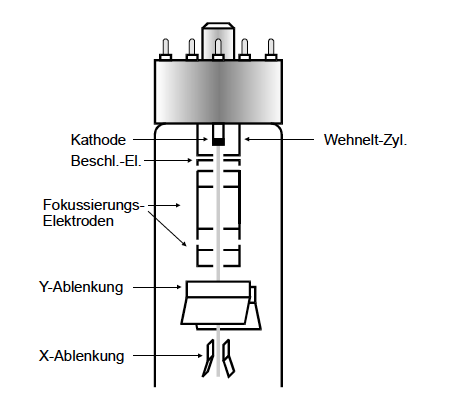
\includegraphics[scale=0.5]{kanone.PNG}
  \caption{Schematischer Aufbau der Kathodenstrahlröhre. \cite{Q1}}
  \label{abb1}
\end{figure}
\FloatBarrier
\subsection{Ablenkungen des Elektronenstrahls im elektrischen Feld}
Passiert ein Elektron ein homogenes elektrisches Feld, so wirkt eine Kraft, die es ablenkt,
weshalb es zu einer Verschiebung des Auftreffpunktes auf dem Detektorschrim kommt.
In Abbildung \ref{abb2} ist der Zusammenhang zwischen der Ablenkspannung, also der Spannung,
die an den Ablenkplatten angelegt wird, und der Verschiebung D des Auftreffpunktes des
Strahls auf dem Schirm zu sehen.
Das elektrische Feld zwischen den beiden Platten kann als homogen betrachtet werden, solange
der Abstand der Platten zueinander im Verhältnis zu deren Länge klein bleibt.
Innerhalb des elektrischen Feldes wirkt dann auf ein Elektron folgende Kraft F:
\begin{align}
  \label{eq1}
  F = e_0 \cdot E = e_0 \frac{U_{\symup{d}}}{d}
\end{align}
\FloatBarrier
\begin{figure}
  \centering
  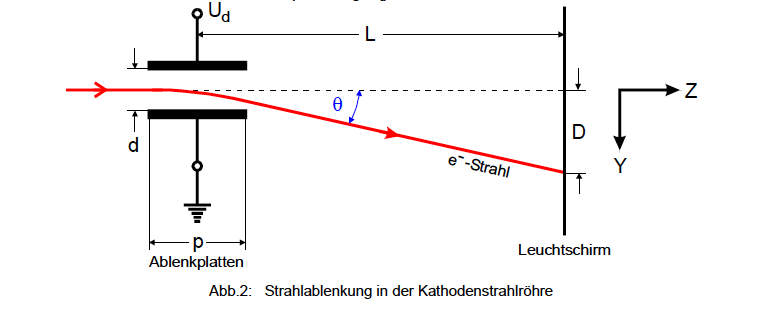
\includegraphics[scale=0.5]{abl.PNG}
  \caption{Schematischer Aufbau der Kathodenstrahlröhre. \cite{Q1}}
  \label{abb2}
\end{figure}
Der Zusammenhang zwischen Ablenkspannung und Verschiebung des Auftreffpunktes ist durch
folgende Gleichung gegeben:
\begin{align*}
  D = \frac{p}{2d} L \frac{U_{\symup{d}}}{U_{\symup{B}}}
\end{align*}
Wobei $p$ die Plattenlänge, $d$ den Plattenabstand, $L$ den Strahlweg und $U_{\symup{B}}$ die Beschleunigungsspannung
beschreiben.
\subsection{Erweiterung der Kathodenstrahlröhre zu einem Kathodenstrahloszillographen}
Soll auf dem Detektorschirm die Zeitabhängigkeit einer angelegten Wechselspannung dargestellt werden,
so wird dazu an die Ablenkplatte, die den Elektronenstrahl in x-richtung ablenkt (horizontal)
eine Sägezahnspannung angelegt. An die Platten, die den Strahl in y-Richtung (vertikal) ablenken,
wird die zu untersuchende Spannung angelegt.
Hierbei ist das Frequenzverhältnis der beiden angelegten Wechselspannungen zueinander von maßgeblicher
Bedeutung. Ist dieses Verhältnis korrekt aufeinander abgestimmt, so ist auf dem Detektorschirm
der zeitliche Verlauf der zu untersuchenden Wechselspannung zu sehen. Hierbei trägt die
angelegte Sägezahnspannung dazu bei, dass die Darstellung der angelegten Wechselspannung
auf dem Detektorschirm zeitlich dargestellt werden kann.
Das zu wählende Verhältnis der beiden Frequenzen ist wie folgt:
\begin{equation*}\label{eq3}
  \symup{n} \nu_{\symup{s}} = \symup{m} \nu_{\symup{w}}  \   ; n,m \in\mathbb{N}
\end{equation*}
Diese Bedingung muss gelten, damit auf dem Schirm stehende Wellen zu sehen sind.
\subsection{Ablenkungen des Elektronenstrahls im magnetischen Feld}
Bewegt sich ein Elektron durch ein magnetisches Feld, so wirkt auf es die Lorentzkraft:
\begin{align}
  \label{eq4}
  F_{\symup{L}} = \symup{q} \vec{\symup{v}} \times \vec{\symup{B}}
\end{align}
Hier ist zu erkennen, dass diese Kraft nur auftritt, wenn die Gewschwindigkeit des Elektrons
eine Komponente besitzt, die senkrecht zum B-Feld steht. Ist $\vec{\symup{v}}$ parallel zu
$\vec{\symup{B}}$, so verschwindet sie.
Der Krümmungsradius der Bahn des abgelenkten Elektrons ergibt sich, wenn die Lorentzkraft
mit der Zentrifugalkraft gleichgesetzt wird, wobei zu beachten ist, dass innerhalb des Magnetfeldes gilt, dass
$v_0 = \big| \vec{v} \big|$ beträgt:
\begin{align}
  \label{eq5}
  r = \frac{m_0 v_0}{e_0 \symup{B}}
\end{align}
Die rechte Seite der Gleichung ist konstant, was zeigt, dass das Elektron auf einer Kreisbahn
abgelenkt wird.
\FloatBarrier
\subsection{Bestimmung der spezifischen Elektronenladung}
Mit dem Versuchsaufbau kann die spezifische Elektronenladung bestimmt werden, indem ein
Elektron mittels einer Kathodenstrahlröhre auf eine konstante Geschwindigkeit $v_0$ beschleunigt wird.
Im Feldfreienraum, flöge es nun geradlinig weiter, bis es auf den Detektroschirm trifft.
Wird mittels eines Helmholtzspulenpaares ein Magnetfeld erzeugt, wird das Elektron, wie zuvor beschrieben, abgelenkt.
Aus Abbildung \ref{abb3} geht hervor, wie der Krümungsradius mit Hilfe des Auftreffpunktes auf dem Detektorschirm
und dem Wirkungsbereich des Magnetfeldes, zu berechnen ist.
\FloatBarrier
\begin{figure}
  \centering
  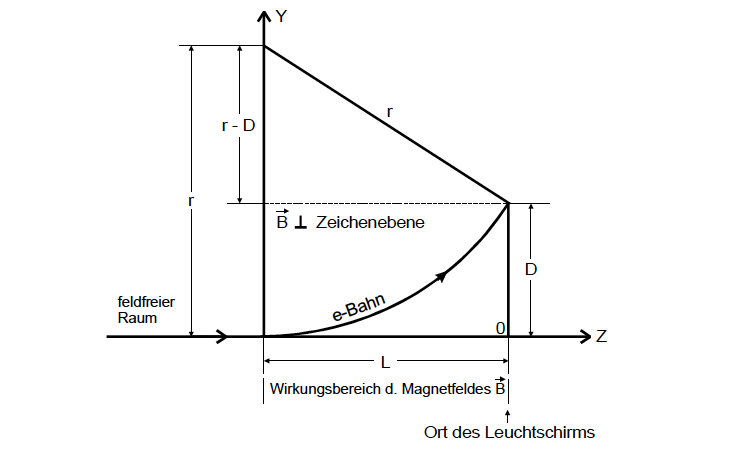
\includegraphics[scale=0.5]{abl2.PNG}
  \caption{Zusammenhang zwischen Auftreffpunkt auf dem Detektorschirm (D),
  Krümmungsradius (r) und Wirkungsbereich des Magnetfeldes (L). \cite{Q1}}
  \label{abb3}
\end{figure}
\FloatBarrier
Mit Hilfe der Formel für die Geschwindigkeit des Elektrons $v_0$, die mittels der Beschleunigungsspannung $U_{\symup{B}}$
berechnet wird:
\FloatBarrier
\begin{align*}\label{eq6}
  v_0 = \sqrt{2 U_{\symup{B}} e_0/m_0}
\end{align*}
\FloatBarrier
und Gleichung \eqref{eq5}, kann dann die spezifische Elektronenladung bestimmt werden:
\FloatBarrier
\begin{align*}
  \frac{e_0}{m_0} = \frac{8 U_{\symup{B}} D^2}{\left(\symup{L}^2 + \symup{D}^2\right)\symup{B}^2}.
\end{align*}
In diesem Verscuh soll außerdem das Erdmagentfeld gemessen werden. Wenn die horizontale Komponente
bekannt ist, kann man durch den Winkel zwischen Erdoberfläche und Magnetfeld den Betrag der Magnetfeldstärke berechnen durchgef
\begin{equation}
  \label{eq:erde}
  B = \frac{B_{\symup{horizontal}}}{\symup{cos}(\phi)} \\
  \end{equation}

\section{Durchführung}
Im ersten Teil des Versuchs wird die Proportionalität zwischen der Ablenkspannung und der
Verschiebung des Auftreffpunktes auf dem Detektorschirm untersucht. Hierbei werden
fünf verschiedene Beschleunigungsspannungen verwendet. Bei denen jeweils die Ablenkspannung
so geregelt wird, dass der Leuchtfleck auf neun verschiedene äquidistante Linien
auf dem Detektorschirm zu sehen ist. Die zugehörigen Spannungen werden notiert.
Die zur Messung gehörige Schaltung ist in Abbildung \ref{abb4} zu sehen.
\begin{figure}
  \centering
  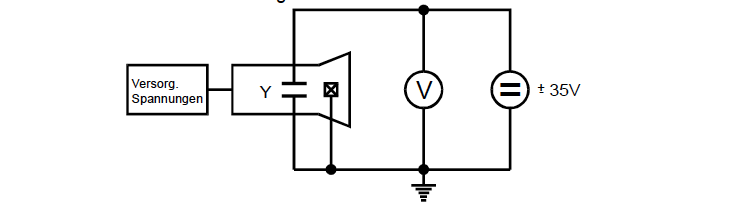
\includegraphics[scale=0.5]{abl3.PNG}
  \caption{Schaltung für die Untersuchung der Proportionalität zwischen Ablenkspannung
  und Verschiebung des Auftreffpunktes. \cite{Q1}}
  \label{abb4}
\end{figure}
\FloatBarrier

\noindent Im zweiten Teil wird ein einfacher Kathodenstrahloszillograph gebaut. Die zugehörige Schaltung
ist in Abbildung \ref{abb5} zu sehen. Hierbei wird die Sägezahnfrequenz so geregelt, dass auf dem Oszillographen
stehende Wellen der Sinusspannung zu sehen sind. Es werden vier verschiedene Vielfache $n$ der
Sägezahnspannung untersucht: $ n = \frac{1}{2}, 1, 2, 3$. Die exakte Frequenz wird am
Frequenzzähler abgelesen. Bei konstanter Beschleunigungsspannung wird des Weiteren die Amplitude
der stehenden Sinuswelle bei allen vier Frequenzvielfachen abgelesen.
\FloatBarrier
\begin{figure}
  \centering
  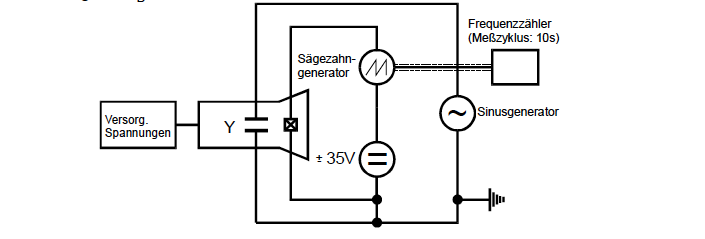
\includegraphics[scale=0.5]{abl4.PNG}
  \caption{Schaltung zum Bau eines einfachen Kathodenstrahloszillographen. \cite{Q1}}
  \label{abb5}
\end{figure}
\FloatBarrier
\noindent Im dritten Teil des Doppelversuchs wird nun die spezifische Elektronenladung
mittels der Ablenkung des Elektronenstrahls im Magnetfeld ermittelt.
Hierzu wird durch eine Helmholtzspule ein homogenes Magnetfeld erzeugt, das senkrecht zur Kathodenstrahlröhre
ausgerichtet wird.
Das entsehende Magnetfeld ist in der Versuchsanleitung \cite{Q1} angegeben:
\begin{equation}
  \label{b-feld}
  B = \mu_0 \frac{8}{\sqrt{125}} \frac{\symup{N} \cdot I }{R}.
\end{equation}
Des Weiteren ist zu beachten, dass die Achse der Kathodenstrahlröhre in Richtung der Horizontalkomponente
des Erdmagnetfeldes ausgerichtet wird. Um die Feldrichtung zu ermitten, steht ein spezieller
Kompass (Deklinatorium/Inklinatorium) bereit.
Anschließend wird bei fünf verschiedenen, konstanten Beschleunigungsspannungen die Strahlverschiebung D
in Abhängigkeit vom, durch den Strom $I$ erzeugten, magnetischen Feld untersucht. Hierzu wird der Strom $I$
neun mal so eingestellt, dass der Auftreffpunkt der Elektonen auf dem Detektorschirm auf neun verschiedenen
äquidistanten Linien zu sehen ist. Der zugehörige Strom zum Auftreffpunkt D werden notiert.

\noindent Im letzten Teil des Versuchs wird die Intensität des Magnetfeldes am Versuchsort ermittelt.
Hierzu wird zunächst der Inklinationswinkel $\varphi$ ermittelt, welcher der Winkel zwischen Horizontalebene
und der Richtung des Erdfeldes ist. Hierzu wird das Inklinatorium um seine vertikale Achso so gedreht, dass
dessen Nadel in Nord-/Südrichtung zeigt. Anschließend wird der Teilkreis des Inklinatoriums um $\SI{90}{\degree}$
gedreht. Nun zeigt die Nadel in Richtung des Erdfeldes. Diese Messung wird dreimal durchgeführt, um eventuelle
Messfehler zu minimieren.
Anschließend wird bei einer konstanten Beschleunigungsspannung und ausgeschaltetem Magnetfeld
die Kathodenstrahlröhre so ausgerichtet, dass sie in die, zuvor mit Hilfe des Inklinatoriums ermittelte,
Nord-/Südrichtung zeigt. Die Lage des Leuchtflecks auf dem Detektorschirm wird exakt notiert und sich gemerkt.
Im Anschluss wird die Versuchsanordnung in Ost-/Westrichtung ausgerichtet, sodass nun das Erdfeld eine
Ablenkung des Elektronenstrahls verursacht. Nun wird die Helmholtzspule angeschaltet und
der Strom $I$ so reguliert, dass das so erzeugte Magnetfeld dem der Erde entgegenwirkt und sich
der Leuchtfleck auf dem Detektorschirm wieder an der gleichen Stelle befindet, wie zu Anfang des Versuchteils.
Der benötigte Strom $I$ wird notiert.


\section{Auswertung}

\subsection{Ablenkung eines Elektronenstrahls im elektrischen Feld}
Im ersten Teil des Versuchs soll die spezifische Ladung eines Elektrons bestimmt werden. Die Messwerte zu dem Versuchsteil
sind in Tabelle \ref{tab:1} aufgelistet. Zur Bestimmung der spezifischen Ladung wird zu jeder Messung eine lineare Regression der Form

\begin{equation*}
  D = a_1 \cdot U_d + C_1
\end{equation*}

durchgeführt, mit

\begin{equation*}
  a_1 = \frac{Lp}{2 d U_b}
\end{equation*}

wobei $D$ die Auslenkung des Elektronenstrahls, $L$ den zurückgelegten Weg des Elektronenstrahls,
$d$ den Abstand der Ablenkplatten, $U_b$ die Beschleunigungsspannung, $U_d$ die Ablenkspannung und $C_1$ den y-Achsenabschnitt beschreibt.
Die Messwerte und die Regressionen sind in Abbildung \ref{abb:1}- \ref{abb:5} dargestellt.


Mit den aus den linearen Regressionen errechneten Steigungen $m$ (Tabelle \ref{tab:2}), lässt sich somit eine weitere
lineare Regression mit den jeweiligen Beschleunigungsspannugen $U_b$ berechnen, mit

\begin{equation*}
  m = a_2 \cdot \frac{1}{U_b} +C_2
\end{equation*}
mit
\begin{equation*}
a_2 = \frac{LP}{2d}
\end{equation*}

der dazu gehörigen linearen Regression in Abbildung \ref{abb:6} folgt für die Röhreneigenschaften $c$

\begin{align*}
  C_2 &= \SI{0.011(10)}{\meter\per\volt} \\
  c_{\symup{gemessen}} &= \frac{pL}{2d} = \SI{-0,3176(29)}{\meter}
\end{align*}

Zum Vergleich des gemessenen Wertes wird der Literaturwert berechnet mit

\begin{align*}
  L &= \SI{14,3}{\centi\meter} + \SI{1,03}{\centi\meter} = \SI{15,33}{\centi\meter} \\
  p &= \frac{1}{2} \cdot (\SI{0,38}{\centi\meter} + \SI{0,95}{\centi\meter}) = \SI{0,665(403)}{\centi\meter} \\
  d &= \SI{1,9}{\centi\meter}
\end{align*}

daraus folgt
\begin{equation*}
  c_{\symup{Literaturwert}} = \frac{pL}{2d} = \SI{0.22(13)}{\meter}
\end{equation*}



\begin{figure}
  \centering
  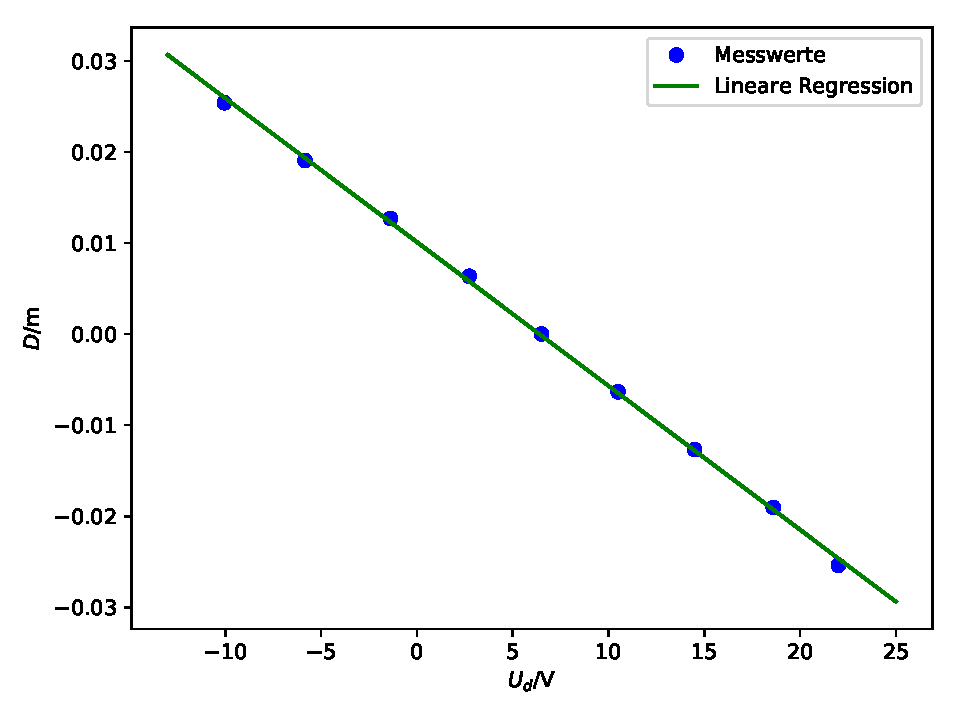
\includegraphics[scale=0.7]{Plot1.1.pdf}
  \caption{Messung 1. $U_b = \SI{200}{\volt}$,  Ablenkspannung $U_d$ , Auslenkung des Elektronenstahls $D$.}
  \label{abb:1}
\end{figure}

\begin{figure}
  \centering
  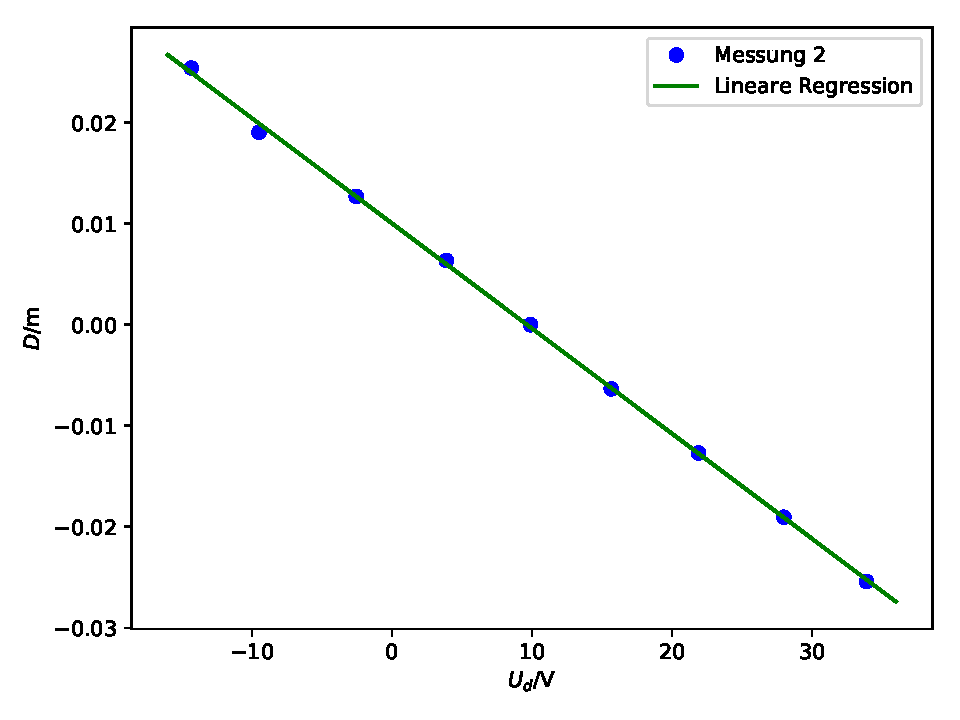
\includegraphics[scale=0.7]{Plot1.2.pdf}
  \caption{Messung 2. $U_b = \SI{300}{\volt}$, Ablenkspannung $U_d$ , Auslenkung des Elektronenstahls $D$.}
  \label{abb:2}
\end{figure}

\begin{figure}
  \centering
  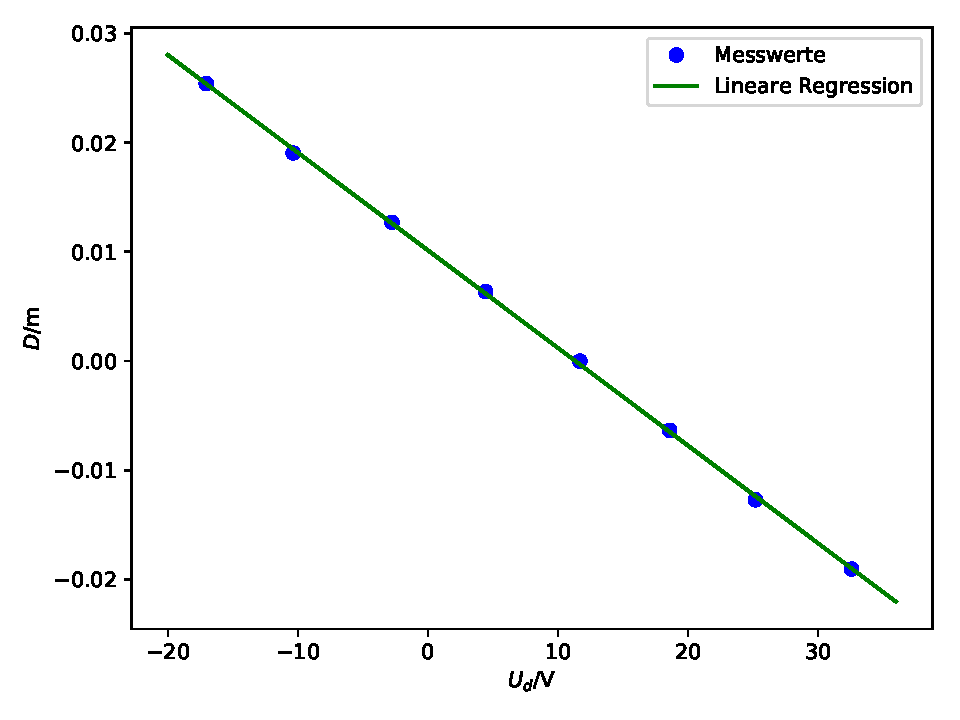
\includegraphics[scale=0.7]{Plot1.3.pdf}
  \caption{Messung 3. $U_b = \SI{350}{\volt}$, Ablenkspannung $U_d$ , Auslenkung des Elektronenstahls $D$.}
  \label{abb:3}
\end{figure}

\begin{figure}
  \centering
  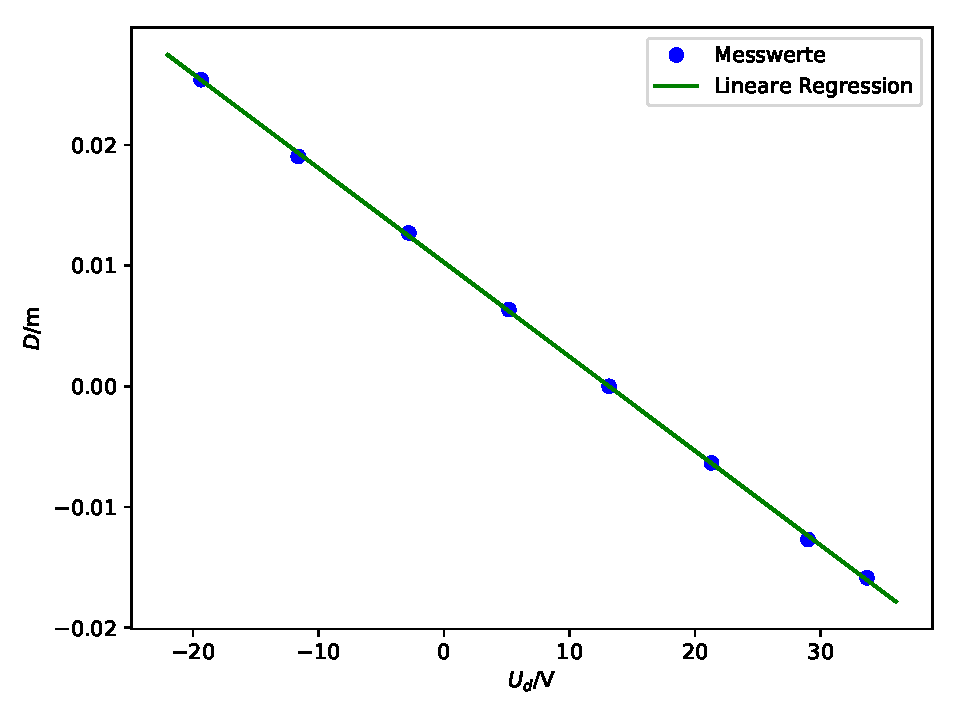
\includegraphics[scale=0.7]{Plot1.4.pdf}
  \caption{Messung 4. $U_b = \SI{400}{\volt}$, Ablenkspannung $U_d$ , Auslenkung des Elektronenstahls $D$.}
  \label{abb:4}
\end{figure}

\begin{figure}
  \centering
  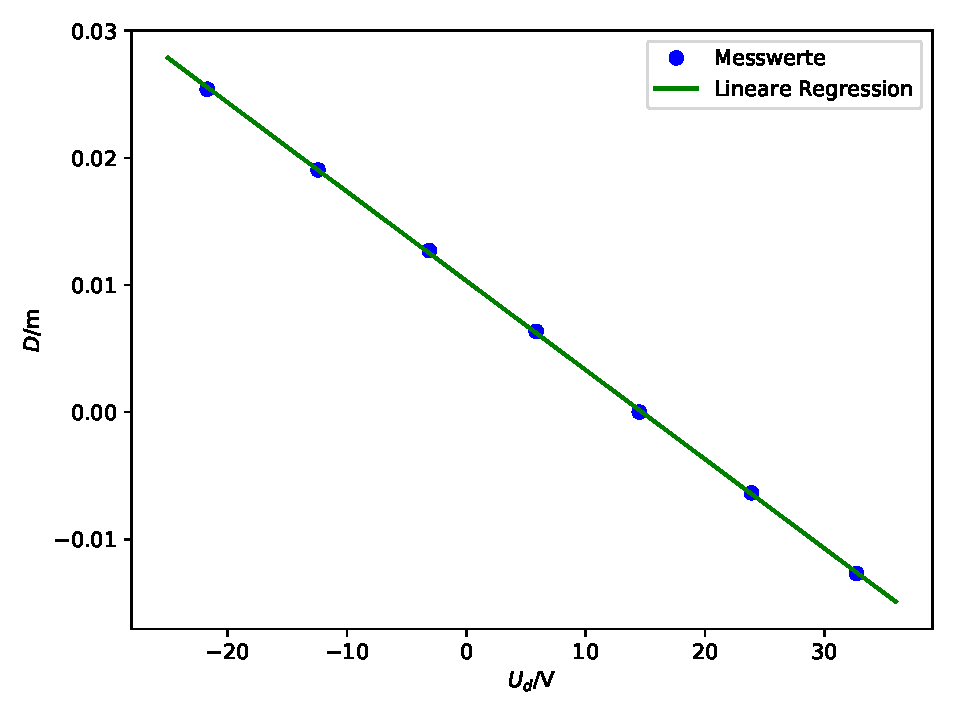
\includegraphics[scale=0.7]{Plot1.5.pdf}
  \caption{Messung 5. $U_b = \SI{450}{\volt}$, Ablenkspannung $U_d$ , Auslenkung des Elektronenstahls $D$.}
  \label{abb:5}
\end{figure}

\begin{table}
  \centering
  \caption{Messwerte der Messung 1-5.}
  \label{tab:1}
  \begin{tabular}{c | c c c c c }
    \toprule
    Ablenkung & \multicolumn{5}{c}{Ablenkspannung} \\
    $D$ / \si{\centi\meter} & $U_{d1}$ / \si{\volt} & $U_{d2}$ / \si{\volt} & $U_{d3}$ / \si{\volt} & $U_{d4}$ / \si{\volt} & $U_{d5}$ / \si{\volt}  \\
    \midrule
    -2,54  & 22,0   & 33,9   & -       & -      & -     \\
    -1,905 & 18,6   & 28,0   & 32,6    & -      & -      \\
    -1,587 & -      & -      & -       & 33,7   & -      \\
    -1,27  & 14,5   & 21,9   & 25,2    & 29,0   & 32,7   \\
    -0,635 & 10,5   & 15,67  & 18,6    & 21,3   & 23,9   \\
    0     & 6,30   & 9,90   & 11,7    & 13,15  & 14,5   \\
    0,635  & 2,73   & 3,89   & 4,44    & 5,17   & 5,86   \\
    1,27   & -1,38  & -2,55  & -2,76   & -2,8   & -3,09  \\
    1,905  & -5,84  & -9,49  & -10,37  & -11,62 & -12,42 \\
    2,54   & -10,05 & -14,33 & -17,05  & -19,35 & -21,7  \\
    \bottomrule
  \end{tabular}
\end{table}

\begin{table}
  \centering
  \caption{Steigungen aus den linearen Regressionen.}
  \label{tab:2}
  \begin{tabular}{c | c c| c }
    \toprule
    Messung & Steigung & y-Achsenabschnitt & Beschleunigungsspannung \\
     & $m$ / \si{\milli\meter\per\volt} & $C_1$ / \si{\centi\meter} & $U_b$ / \si{\volt} \\
    \midrule
    1 & \num{-1,580(15)} & \num{1,010(19)}  &  200 \\
    2 & \num{-1,040(9)} &  \num{1,004(16)}  & 300 \\
    3 & \num{-0,894(6)} &  \num{1,014(10)}  & 350 \\
    4 & \num{-0,781(4)} &  \num{1,026(9)}  & 400 \\
    5 & \num{-0,702(3)} &  \num{1,033(6)}  & 450 \\
    \bottomrule
  \end{tabular}
\end{table}

\begin{figure}
  \centering
  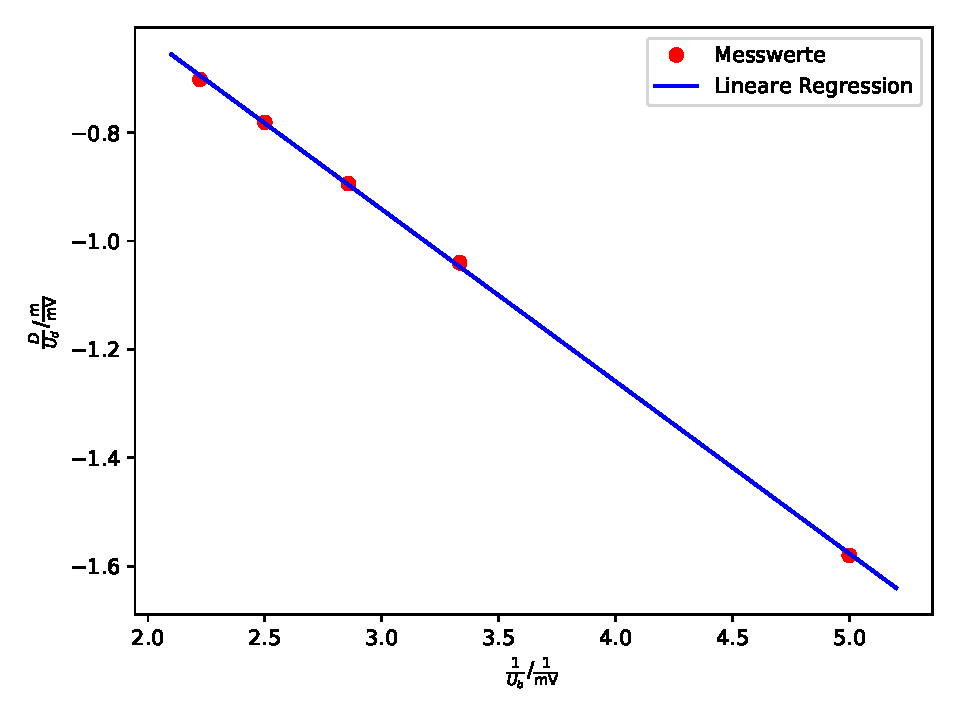
\includegraphics[scale = 0.7]{PlotSteigung1.pdf}
  \caption{Lineare Regression. Beschleunigungsspannung $U_b$, Ablenkung $D$, Ablenkspannung $U_d$.}
  \label{abb:6}
\end{figure}

Außerdem soll nun die Frequenz der Sinusschwingung einer Kathodenstrahlröhre mit Hilfe der Frequenz der Sägezahnspannung
berechnet werden, dazu wird folgende Relation für stehende Wellen bei einer Kathodenstrahlröhre verwendet:

\begin{equation}
  \label{re:v}
   \nu_{\symup{Sinus}} = n \cdot \nu_{\symup{Saegezahn}}
\end{equation}

Durch Einsetzen der Messwerte für $\nu_{\symup{Saegezahn}}$ und $n$ aus Tabelle \ref{tab:3} erhält man die Frequenzen der
Sinusspannung $\nu_{\symup{Sinus}}$.

\begin{table}
  \centering
  \caption{Messung der Frequenzen der Sägezahnspannung.}
  \label{tab:3}
  \begin{tabular}{c c | c}
    \toprule
    Frequenz der & Proportionalitäts- & Frequenz der \\
    Sägezahnspannung & faktor & Sinusspannung \\
    $\nu_{\symup{Saegezahn}}$ / \si{\hertz} & $n$ & $\nu_{\symup{Sinus}}$ / \si{\hertz} \\
    \midrule
    79.92 & 1 & 79,92 \\
    159.77 & 0,5 & 79,885 \\
    39.90 & 2 & 79,8 \\
    26.66 & 3 & 79,98 \\
    \bottomrule
  \end{tabular}
\end{table}

Durch die Berechnung des Mittelwertes und der Standardabweichung, folgt für die Frequenz der Sinusspannung

\begin{equation*}
  \nu_{\symup{Sinus}} = \SI{79.896(37)}{\hertz}
\end{equation*}

Zuletzt soll aus diesem Versuchsteil die maximale Spannung der Ablenkplatten bestimmt werden. Hierzu wird die vorherige Messung mit
der Beschleunigunsspannung

\begin{equation*}
  U_b = \SI{350}{\volt}
\end{equation*}
 benötigt, denn die berechneten Röhreneigenschaften liegen bei

\begin{equation*}
  c = \SI{-0,3176(29)}{\meter}.
\end{equation*}

Mit dem Mittelwert der gemessenen Amplituden aus Tabelle \ref{tab:amplitude} und der Gleichung

\begin{align*}
  A &= \SI{1,09(07)}{\centi\meter} \\
  A &= \frac{c}{U_b} U_d
\end{align*}

folgt für die Ablenkspannung

\begin{equation*}
  U_d = \frac{A U_b}{c} = \SI{-12,0(8)}{\volt}
\end{equation*}

\begin{table}
  \centering
  \caption{Amplituden des Kathodenstraloszillographen.}
  \label{tab:amplitude}
  \begin{tabular}{c c}
    \toprule
    Proportionalitätsfaktor & Amplitude \\
    $n$ & $A$ / \si{\centi\meter}\\
    \midrule
    1 & 1,03 \\
    0,5 & 0,95 \\
    2 & 1,11 \\
    3 & 1,27 \\
    \bottomrule
  \end{tabular}
\end{table}


\subsection{Ablenkung eines Elektronenstrahls im transversalen Magnetfeld}

Zur Bestimmung der spezifischen Ladung von Elektronen wird eine lineare Regression der Form

\begin{equation*}
  \frac{D}{D²+L²} = a_3 \cdot B + C_3
\end{equation*}

durchgeführt, mit

\begin{equation}
  a_3 = \frac{1}{\sqrt{8 U_b}} \sqrt{\frac{e_0}{m_0}}
\end{equation}

wobei $D$ die Auslenkung des Elektronenstrahls, $L$ die Länge des Elektronenstrahls durch das Magnetfeld, $U_b$ die Beschleunigunsspannung,
$e_0$ die Elementarladung eines Elektrons, $m_0$ die Masse eines Elektrons, $B$ das Magnetfeldstärke und $C_3$ den y-Achsenabschnitt beschreibt.

Die Messwerte und die aus der Stromstärke $I$ berechneten Magnetfelder sind in Tabelle \ref{tab:4} und \ref{tab:5} aufgelistet, zur Berechnung der Magnetfeldstärken
wird die Formel \eqref{b-feld} für das Magnetfeld einer Helmholtz-Spule verwendet.

\begin{table}
  \centering
  \caption{Messwerte zur Bestimmung der spezifischen Ladung.}
  \label{tab:4}
  \begin{tabular}{c c c c}
    \toprule
    Ablenkung & Stromstärke des Magnetfeldes & Magnetfeldstärke & \\
    $D$ / \si{\centi\meter} & $I$ / \si{\ampere} & $B$ / \si{\milli\tesla} & $\frac{D}{L²+D²}$ / \si{\centi\meter} \\
    \midrule
    \multicolumn {4}{c}{Messung 1, $U_b$ = \SI{200}{\volt}} \\
    \midrule
    2,54 & 0 & 0 & 81,23\\
    1,905 & 0,26 & 16,58 & 61,48 \\
    1,27 & 0,57 & 36,35 & 41,25\\
    0,635 & 0,90 & 57,39 & 20,71 \\
    0      & 1,15 & 73,34 & 0 \\
    -0,635 & 1,45 & 92,47 & -20,71 \\
    -1,27  & 1,80 & 114,79 & -41,25 \\
    -1,905 & 2,10 & 133,92 & -61,48 \\
    -2,54  & 2,40 & 153,05 & 81,23 \\
    \midrule
    \multicolumn {4}{c}{Messung 2, $U_b$ = \SI{300}{\volt}} \\
    \midrule
    2,54 & 0 & 0 & 81,23 \\
    1,905 & 0,36 & 22,95 & 61,48 \\
    1,27 & 0,72 & 45,92 & 41,25 \\
    0,635 & 1,10 & 70,15 & 20,71 \\
    0      & 1,45 & 92,47 & 0 \\
    -0,635 & 1,85 & 117,98 & -20,71 \\
    -1,27 & 2,25 & 143,49 & -41,25 \\
    -1,905 & 2,60 & 165,81 & -61,48 \\
    -2,54 & 3,00 & 191,31 & -81,23 \\
    \midrule
    \multicolumn {4}{c}{Messung 3, $U_b$ = \SI{350}{\volt}} \\
    \midrule
    2,54 & 0  & 0 & 81,23 \\
    1,905 & 0,36 & 22,95 & 61,48 \\
    1,27 & 0,78 & 49,74 & 41,24 \\
    0,635 & 1,20  & 76,53 & 20,71 \\
    0      & 1,55 & 98,85 & 0 \\
    -0,635 & 2,00 & 127,54 & -20,71 \\
    -1,27 & 2,40 & 153,05 & -41,25 \\
    -1,905 & 2,85 & 181,75 & -61,48  \\
    -2,54 & 3,25  & 207,56 & -81,23\\
    \midrule
    \multicolumn {3}{c}{Messung 4, $U_b$ = \SI{400}{\volt}} \\
    \midrule
    2,54 & 0  & 0  & 81,23 \\
    1,905 & 0,39  & 24,87 & 61,48 \\
    1,27 & 0,84  & 53,56 & 41,25 \\
    0,635 & 1,25  & 79,71 & 20,71 \\
    0      & 1,60 &  102,03 & 0 \\
    -0,635 & 2,10 &  133,92 & -20,71  \\
    -1,27 & 2,50 & 159,42 & -41,25 \\
    -1,905 & 3,00 &  191,31 & -61,48 \\
    \bottomrule
  \end{tabular}
\end{table}

\begin{table}
  \centering
  \caption{Messwerte zur Bestimmung der spezifischen Ladung.}
  \label{tab:5}
  \begin{tabular}{c c c c}
    Ablenkung & Stromstärke des Magnetfeldes & Magnetfeldstärke &  \\
    $D$ / \si{\centi\meter} & $I$ / \si{\ampere} & $B$ / \si{\milli\tesla} & $\frac{D}{L²+D²}$ / \si{\centi\meter} \\
    \midrule
    \multicolumn {4}{c}{Messung 5, $U_b$ = \SI{250}{\volt}} \\
    \midrule
    2,54 & 0 & 0 & 81,23 \\
    1,905 & 0,30 & 19,13 & 61,48 \\
    1,27 & 0,64 & 40,81 & 41,25  \\
    0,635 & 1,00 & 63,77 & 20,71 \\
    0      & 1,39 & 88,64 & 0 \\
    -0,635 & 1,65 & 105,22 & -20,71\\
    -1,27 & 2,00 & 127,54 & -41,25 \\
    -1,905 & 2,40& 153,05 & -61,48 \\
    -1,905 & 2,70 & 172,18 & -81,23 \\
    \bottomrule
  \end{tabular}
\end{table}

\begin{figure}
  \centering
  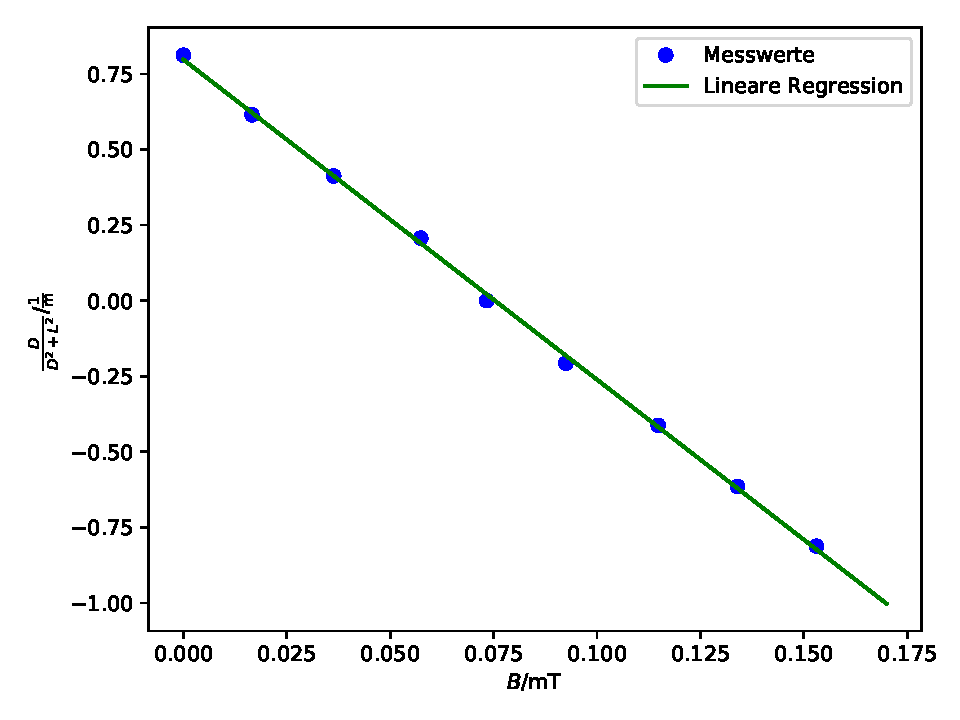
\includegraphics[scale = 0.7]{Plot2.1.pdf}
  \caption{Messung 1. $ U_b = \SI{200}{\volt}$, Magnetfeldstärke $B$ , Auslenkung des Elektronenstahls $D$, Länge des Elektronenstrahls im Magnetfeld $L$}
  \label{abb:7}
\end{figure}
\begin{figure}
  \centering
  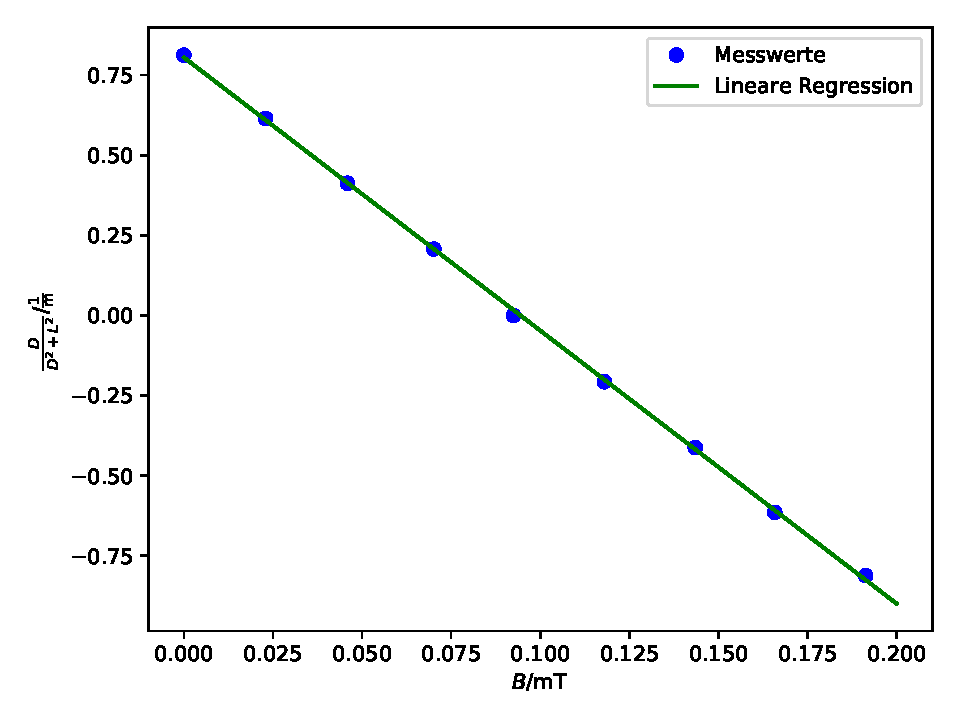
\includegraphics[scale = 0.7]{Plot2.2.pdf}
  \caption{Messung 2. $ U_b = \SI{300}{\volt}$, Magnetfeldstärke $B$ , Auslenkung des Elektronenstahls $D$, Länge des Elektronenstrahls im Magnetfeld $L$}
  \label{abb:8}
\end{figure}
\begin{figure}
  \centering
  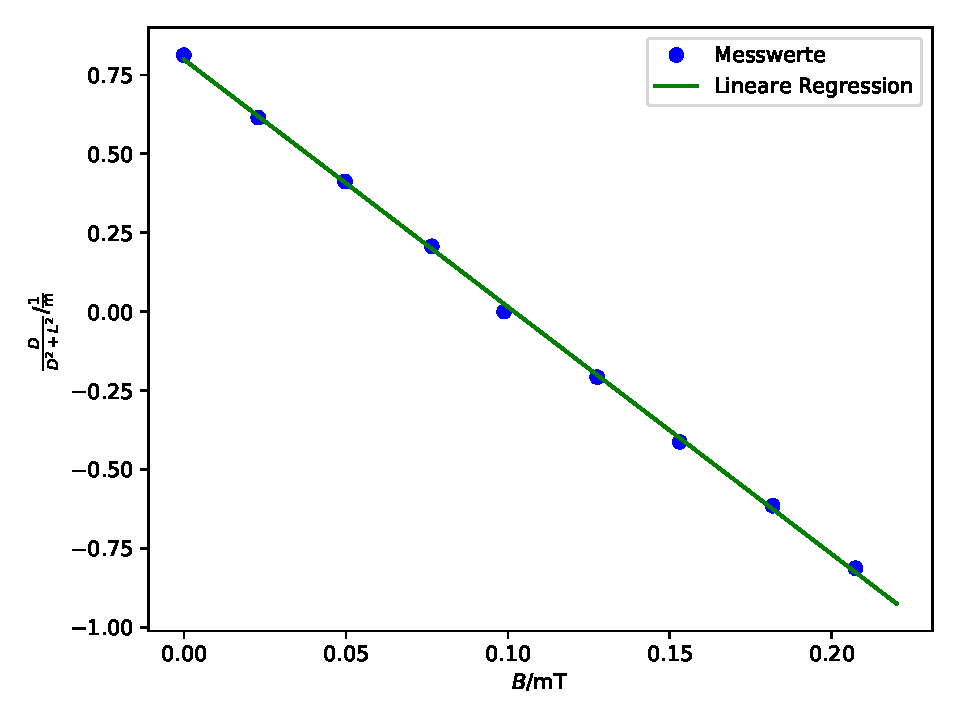
\includegraphics[scale = 0.7]{Plot2.3.pdf}
  \caption{Messung 3. $ U_b = \SI{350}{\volt}$, Magnetfeldstärke $B$ , Auslenkung des Elektronenstahls $D$, Länge des Elektronenstrahls im Magnetfeld $L$}
  \label{abb:9}
\end{figure}
\begin{figure}
  \centering
  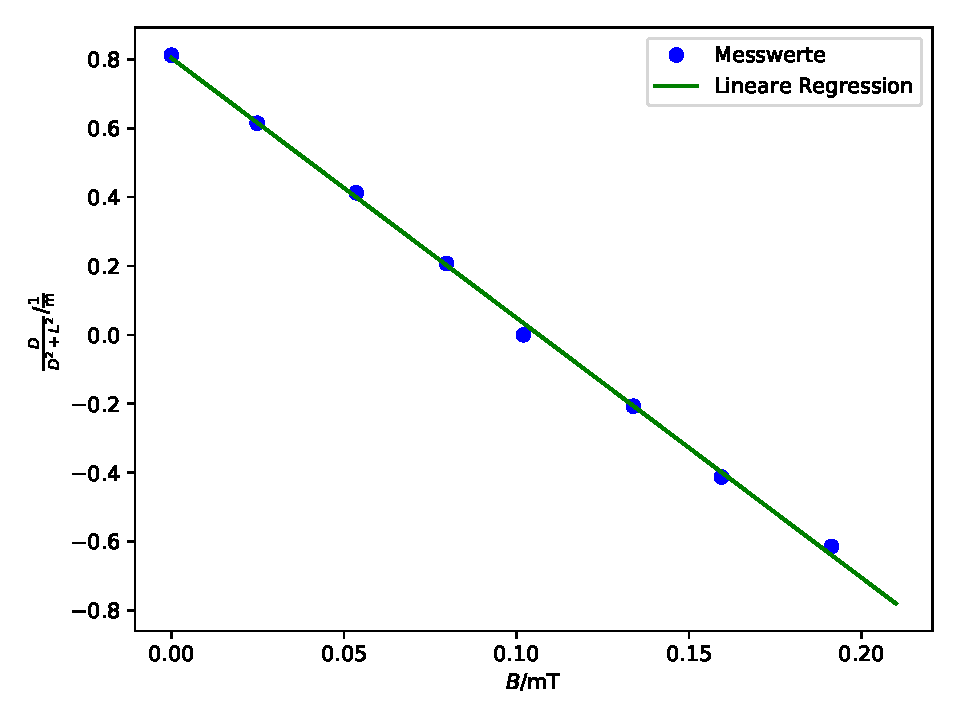
\includegraphics[scale = 0.7]{Plot2.4.pdf}
  \caption{Messung 4. $ U_b = \SI{400}{\volt}$, Magnetfeldstärke $B$ , Auslenkung des Elektronenstahls $D$, Länge des Elektronenstrahls im Magnetfeld $L$}
  \label{abb:10}
\end{figure}
\begin{figure}
  \centering
  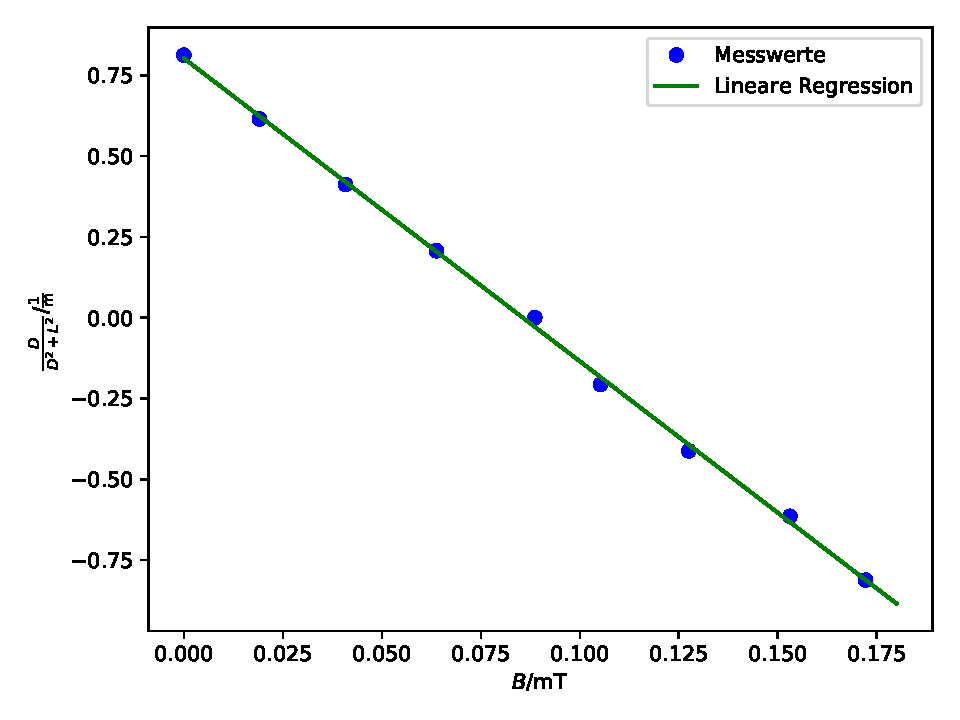
\includegraphics[scale = 0.7]{Plot2.5.pdf}
  \caption{Messung 5. $ U_b = \SI{250}{\volt}$, Magnetfeldstärke $B$ , Auslenkung des Elektronenstahls $D$, Länge des Elektronenstrahls im Magnetfeld $L$}
  \label{abb:11}
\end{figure}


Aus den Linearen Regressionen werden die Steigungen $m$ und der y-Achsenabschnitt $c$ zu jeder Messung mit den unterschiedlichen
Bremsspannungen $U_b$ berechnet, diese sind in Tabelle \ref{tab:6} aufgelistet.


\begin{table}
  \centering
  \caption{Steigungen und y-Achsenabschnitte zu den jeweiligen Bremsspannungen.}
  \begin{tabular}{c | c c}
    \toprule
    Bremsspannung & Steigung & y-Achsenabschnitt \\
    $U_b$ / \si{\volt} & $m$ / \si{\sqrt{\kilo\coulomb\per\gram\volt}} & $C_3$ / \si{\meter} \\
    \midrule
    200 & \num{-10,59(11)} & \num{0,798(10)} \\
    300 & \num{-8,52(5)}   & \num{0,805(6)} \\
    350 & \num{-7,83(7)}   & \num{0,799(8)} \\
    400 & \num{-7,55(11)}  & \num{0,804(12)} \\
    250 & \num{-9,38(11)}  & \num{0,803(11)} \\
    \bottomrule
  \end{tabular}
  \label{tab:6}
\end{table}

Aus den Steigungen $m$ wird eine weitere lineare Regression in Abhängigkeit von $\frac{1}{U_b}$ der Form

\begin{equation*}
  m = a_4 \cdot \frac{1}{U_b} + C_4
\end{equation*}

durchgeführt, mit
\begin{equation}
  a_4 = \sqrt{\frac{e_0}{8m_0}}
\end{equation}

\begin{figure}
  \centering
  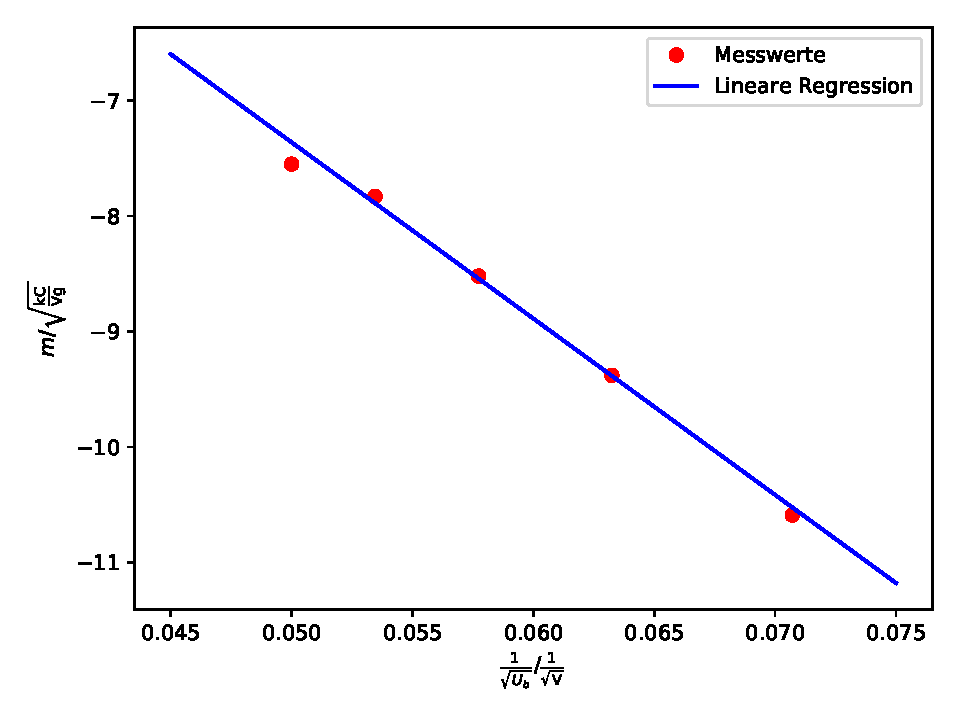
\includegraphics[scale = 0.7]{PlotSteigung2.pdf}
  \caption{Lineare Regression. Beschleunigungsspannung $U_b$, Steigung $m$.}
  \label{abb:11}
\end{figure}

\begin{align*}
  s &= \sqrt{\frac{e_0}{8m_0}} = \SI{-1,53(7)e5}{\sqrt{\coulomb\per\kilo\gram}} \\
  C_4 &= \SI{3(4)e2}{\sqrt{\coulomb\per\kilo\gram\volt}}
\end{align*}

Aus der Steigung $s$ lässt sich nun durch Umformen die spezifische Ladung $\frac{e_0}{m_0}$ bestimmen:

\begin{equation*}
  \frac{e_0}{m_0} = 8s² = \SI{1.87(18)e11}{\coulomb\per\kilo\gram}
\end{equation*}

Zur Berechnung des Erdmagnetfelds wird das Gegenmagnetfeld berechnet, welches durch die Helmholtz-Spule erzeugt wird.
Das Magnetfeld der Spule wird durch die Formel \ref{eq:Spule} berechnet. Mit einer Stromstärke von

\begin{equation*}
  I = \SI{195}{\milli\ampere}
\end{equation*}
 folgt für die Magnetfeldstärke
 \begin{equation*}
   B = \SI{12,435}{\micro\tesla}
 \end{equation*}

 Da dies aber nur der horizontale Komponente des Magnetfelds entspricht, wird der Erdmagnetfeld über den gemessenen Winkel berechnet.
 Die gemessenen Winkel zwischen der Erdoberfläche und der Ausrichtung des Magnetfelds sind in Tabelle \ref{tab:7} aufgelistet.

 \begin{table}
   \centering
   \caption{Messung des Winkels zwischen der Erdoberfläche und des Magnetfelds.}
   \begin{tabular}{c}
     \toprule
     Winkel\\
     $\phi$ / \si{\degree} \\
     \midrule
     71 \\
     73 \\
     65 \\
     \bottomrule
   \end{tabular}
   \label{tab:7}
 \end{table}

 Durch Berechnung des Mittelwertes und der Standardabweichung folgt für den Winkel $\phi$

 \begin{equation*}
   \phi = \SI{69,667(3205)}{\degree}
 \end{equation*}

Mit der Gleichung \eqref{eq:erde} und
 \begin{align*}
   \Delta B &= \frac{B_{\symup{horizontal}}\symup{sin}(\phi)}{\symup{cos²}(\phi)} \cdot \Delta \phi
 \end{align*}

 folgt für das Magnetfeld der Erde

 \begin{equation*}
   B = \SI{38,196(5767)}{\micro\tesla}.
 \end{equation*}

 \section{Diskussion}

Die Messung der Empfindlichkeit $c$ der Kathodenstrahlröhre ergibt folgenden Wert im Vergleich zu dem Literaturwert
\begin{align*}
  c_{\symup{gemessen}} &= \SI{-0,3176(29)}{\meter} \\
  c_{\symup{Literaturwert}}& = \SI{0.22(13)}{\meter}.
\end{align*}
Das Vorzeichen der Ergebnisse kann hierbei irgnoriert werden, da wir die Spannung anders herum angeschlossen haben und wir somit
eine vom Vorzeichen veränderte Spannung erhalten haben. Vom Betrag her macht dies aber keinen Unterschied. Die Relative Abweichung
ist mit
\begin{equation*}
  p_c = \frac{c_{\symup{gemessen}}}{c_{\symup{Literaturwert}}} -1 = \SI{44.36}{\percent}
\end{equation*}
recht hoch. Dies lässt sich unter anderem auch auf die Berechnung des Literaturwertes zurückführen, da zum berechnen
des Abstandes der Kondensatorplatten ein gemittelter Wert genommen wurde und dieser in die Formel eines Plattenkondensators mit parallelen
Platten eingesetzt wurde. In diesem Versuchsaufbau hatten wir aber einen Plattenkondensator, dessen Plattenabstand ab ungefähr der Mitte immer
größer wurde. Dies führt zu einem Fehler in der Berechnung des Literaturwertes.

Die gemessene spezifische Ladung eines Elektrons

\begin{align*}
  \left( \frac{e_0}{m_0} \right)_{\symup{gemessen}} &= \SI{1.87(18)e11}{\coulomb\per\kilo\gram} \\
  \left( \frac{e_0}{m_0} \right)_{\symup{Literaturwert}} &= \SI{1,759e11}{\coulomb\per\kilo\gram} \\
\end{align*}

hat im Vergleich zu dem Literaturwert nur eine sehr geringe Abweichung von

\begin{equation*}
  p_{\frac{e_0}{m_0}} = \frac{\left( \frac{e_0}{m_0} \right)_{\symup{gemessen}}}{\left( \frac{e_0}{m_0} \right)_{\symup{Literaturwert}}} -1 = \SI{6,31}{\percent}.
\end{equation*}

Eine Fehlerquelle des Versuchs könnte das Amperemeter sein, da dies teilweise beim Übergang in eine andere Größenodnung leicht unterschiedliche
Werte angezeigt hat.

Die Messung des Erdmagnetfeldes auf der Erdoberfläche ergibt folgenden Wert im Vergleich zum Literaturwert

\begin{align*}
  B_{\symup{gemessen}} &= \SI{38,196(5767)}{\micro\tesla} \\
  B_{\symup{Literaturwert}} &  \approx \SI{48}{\micro\tesla} \\
\end{align*}

Die Abweichung vom Literaturwert beträgt

\begin{equation*}
  p_B = 1- \frac{B_{\symup{gemessen}}}{B_{\symup{Literaturwert}}} = \SI{20,48}{\percent}
\end{equation*}

Die Abweichung lässt sich auf die ungenaue Messung des Winkels $\phi$ zurückführen, welche mit einem alten, nicht mehr ganz genau funktionierenden
Kompass durchgeführt wurde, da die Nadel sich nicht mehr frei im Kompass bewegen konnte. Somit hat sich auch die Apperatur nicht genau nach
Norden ausrichten lassen. Außerdem wurde die Messung mit einer zu hohen Beschleunigunsspannung durchgeführt.

\nocite{*}
\printbibliography
